\documentclass{article}
    \usepackage{amssymb}
    \usepackage[utf8]{inputenc}
    \usepackage[russian]{babel}
    \usepackage[left=2cm,right=2cm,
        top=2cm,bottom=2cm,bindingoffset=0cm]{geometry}
    \usepackage{hyperref}
    \hypersetup{
        colorlinks=true,
        linkcolor=blue,
        filecolor=magenta,      
        urlcolor=cyan,
    }
  \usepackage{graphicx}
  \usepackage{booktabs}
  \usepackage{hyperref}
  \graphicspath{{pictures/}}
  \DeclareGraphicsExtensions{.pdf,.png,.jpg}
\usepackage{subcaption}
%\captionsetup{compatibility=false}

\begin{document}
\begin{center}{\hugeОтчет по дипломной работе за неделю\\}\end{center}
Дата: 25.3.2021\\
Научные руководители: Герасимов С.В., Мещеряков А.В.\\
Студент: Немешаева Алиса\\
Курс: 4\\

\renewcommand{\labelitemi}{$\blacksquare$}
\renewcommand\labelitemii{$\square$}
\begin{enumerate}
    \item Построены гистограммы ~\ref{Fig:Hist}{} для оценки количества ложных источников в 
        полученных каталогах. 
        Чтобы построить такие гистограммы, потребовалось сделать следующее:\\
        \begin{itemize}
            \item Создаем координаты для детектированного каталога и для ground truth каталога.\\
            \item Сопоставляем координаты: для каждого объекта из детектированного каталога находим
                ближайшее скопление из gt-каталога.\\
            \item В детектированном каталоге есть объекты, для которых в радиусе  
                $(400^{\prime \prime})$ найдено скопление в gt-каталоге - это красная выборка (те
                скопления, большую часть которых мы считаем true positive).\\
            \item Из gt-каталога исключаем те объекты, которые были сопоставлены с объектами из
                детектированного каталога в предыдущем пункте.\\
            \item Снова сопоставляем координаты детектированного каталога с новой версией 
                gt-каталога: теперь мы выбираем те объекты, для которых ближйшее скопление 
                находится в промежутке $(400^{\prime \prime}, 1500^{\prime \prime}]$ - это синяя 
                выборка (объекты, чьё количество поможет оценить содержание ложных объектов в 
                каталоге).\\
            \item Строим гистограммы по синим и красным выборкам для разных ground truth каталогов.\\
        \end{itemize}
    \item Такие графики позволяют отслеживать динамику количества ложных срабатываний относительно 
        параметра max\_pred у обнаруженных объектов. Так, создавая урезанный по max\_pred  
        ~\ref{Fig:Hist6} каталог, мы можем оценить примерное количество истинных и ложных 
        скоплений.\\
    \item Построены карты для валидационных карт с сопоставлением детектированных каталогов и 
        ground truth каталогов:\\
        \begin{itemize}
            \item Все доступные каталоги:~\ref{Fig:Map_All}\\
            \item Только PSZ2:~\ref{Fig:Map_PSZ2}\\
            \item Только ACT:~\ref{Fig:Map_ACT}{}\\
        \end{itemize}
    \item Эти карты позволяют оценить область покрытия различных каталогов. Например, четко видны 
        границы видимости для каталога ACT.\\
\end{enumerate}




\begin{figure}[h]
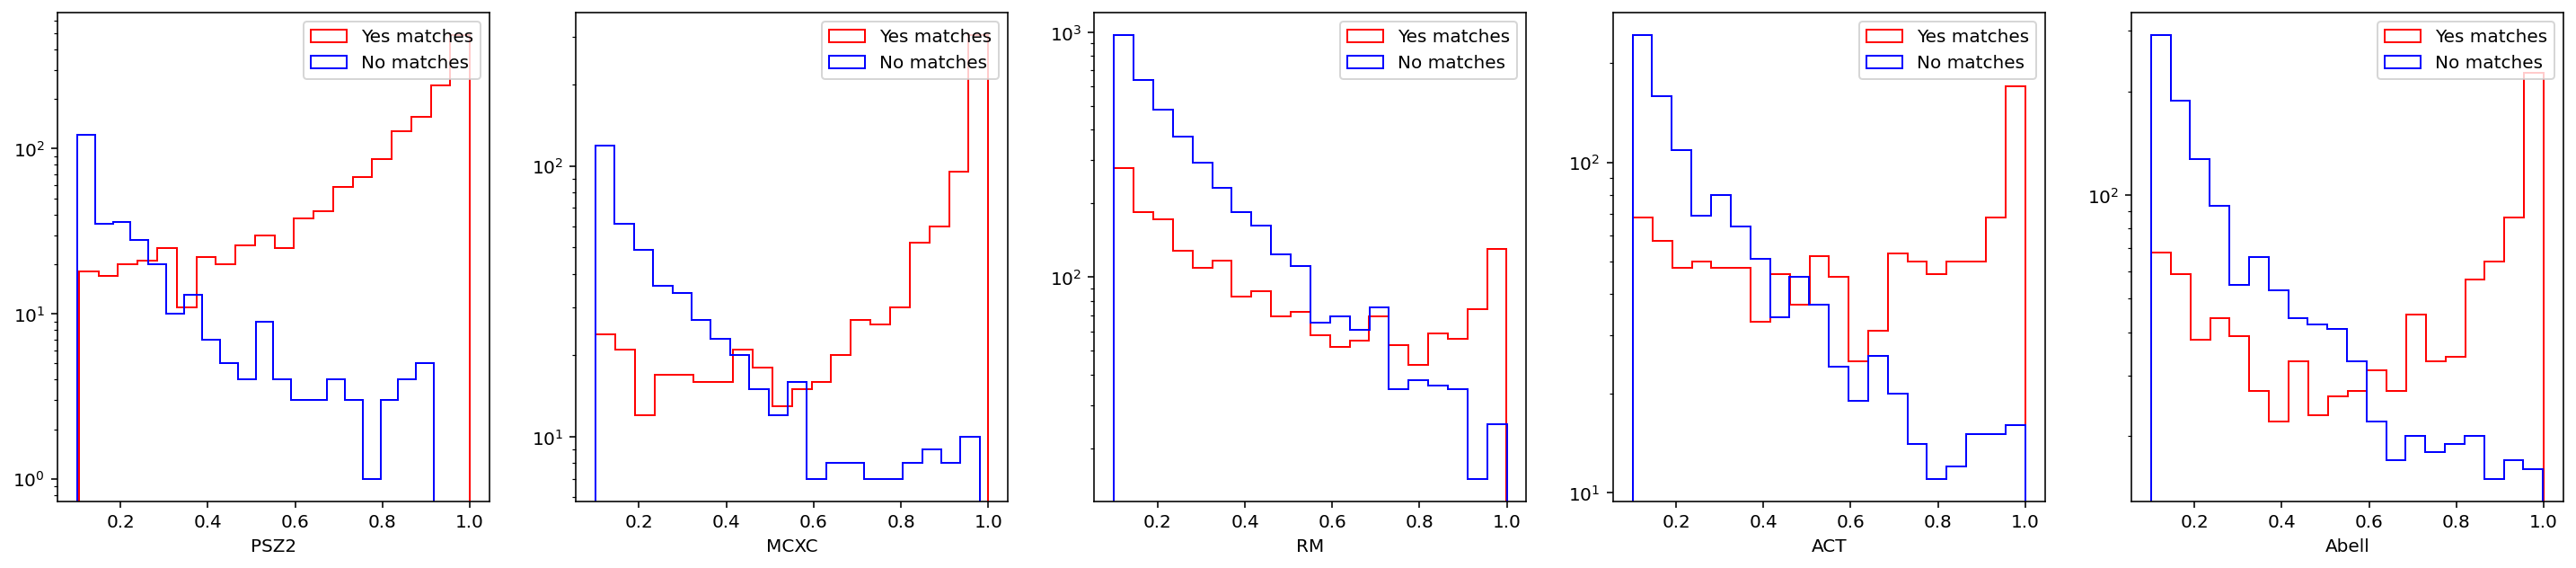
\includegraphics[width=\linewidth]{2circles_histogram}
\caption{Гистограммы для оценки количества ложных источников в детектированном каталоге.}
\label{Fig:Hist}
\end{figure}

\begin{figure}[h]
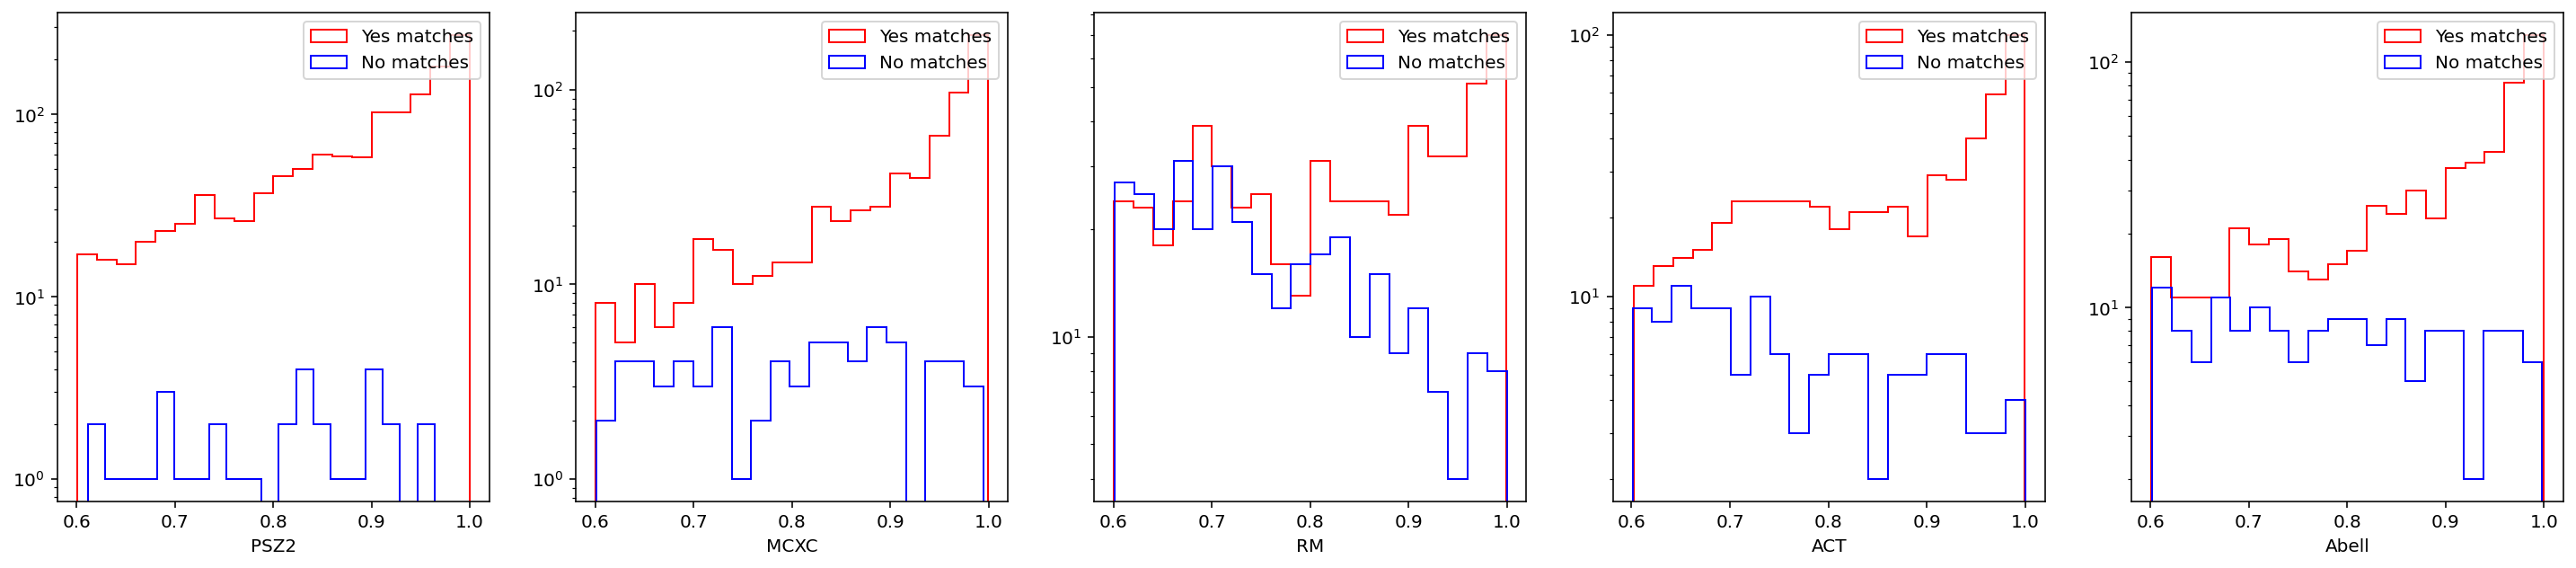
\includegraphics[width=\linewidth]{2circles_histogram_06}
\caption{Гистограммы для оценки количества ложных источников в детектированном каталоге с 
    $max\_pred \geqslant 0.6$.}
\label{Fig:Hist6}
\end{figure}

\begin{figure}[h]
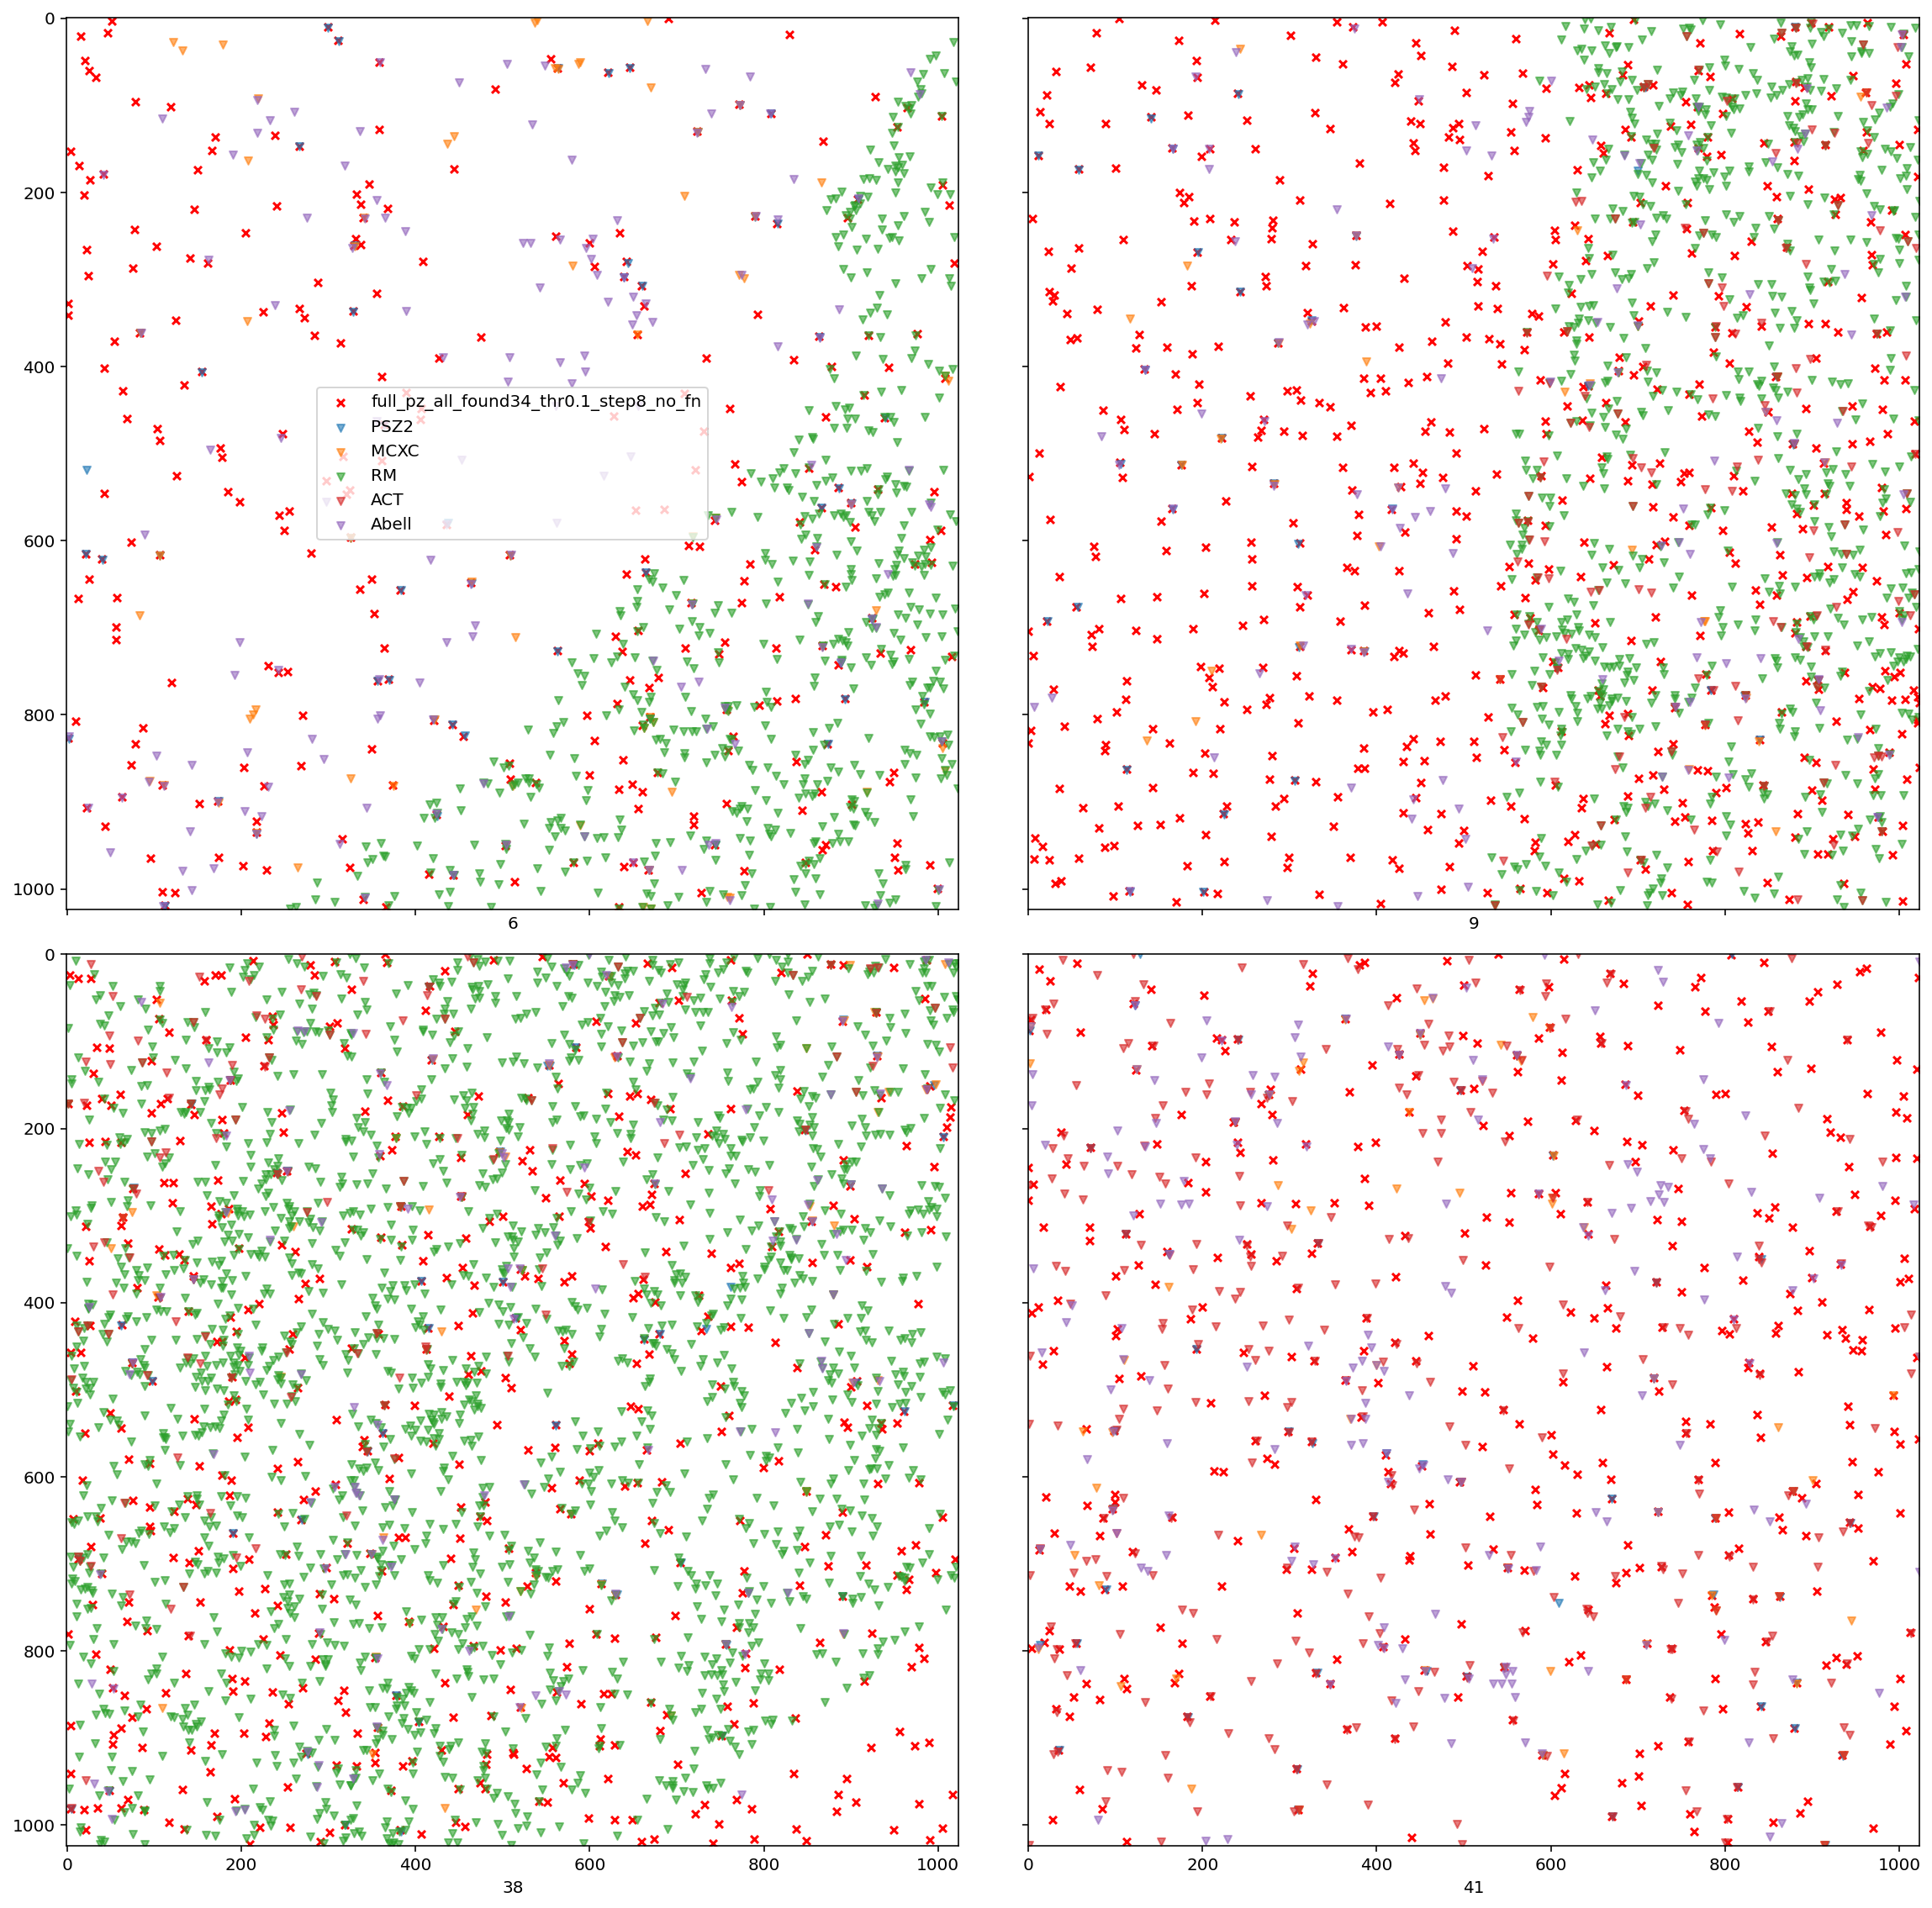
\includegraphics[width=\linewidth]{map_all}
\caption{Карта распределения объектов из детектированного каталога и скоплений из ground truth 
    каталогов (PSZ2, MCXC, RedMaPPer, Abell, ACT), пиксели из разбиения $n_{side}=2$ с номерами
    $[6, 38]$ (левая колонка - восток) и $[9, 41]$ (правая колонка - запад)}
\label{Fig:Map_All}
\end{figure}

\begin{figure}[h]
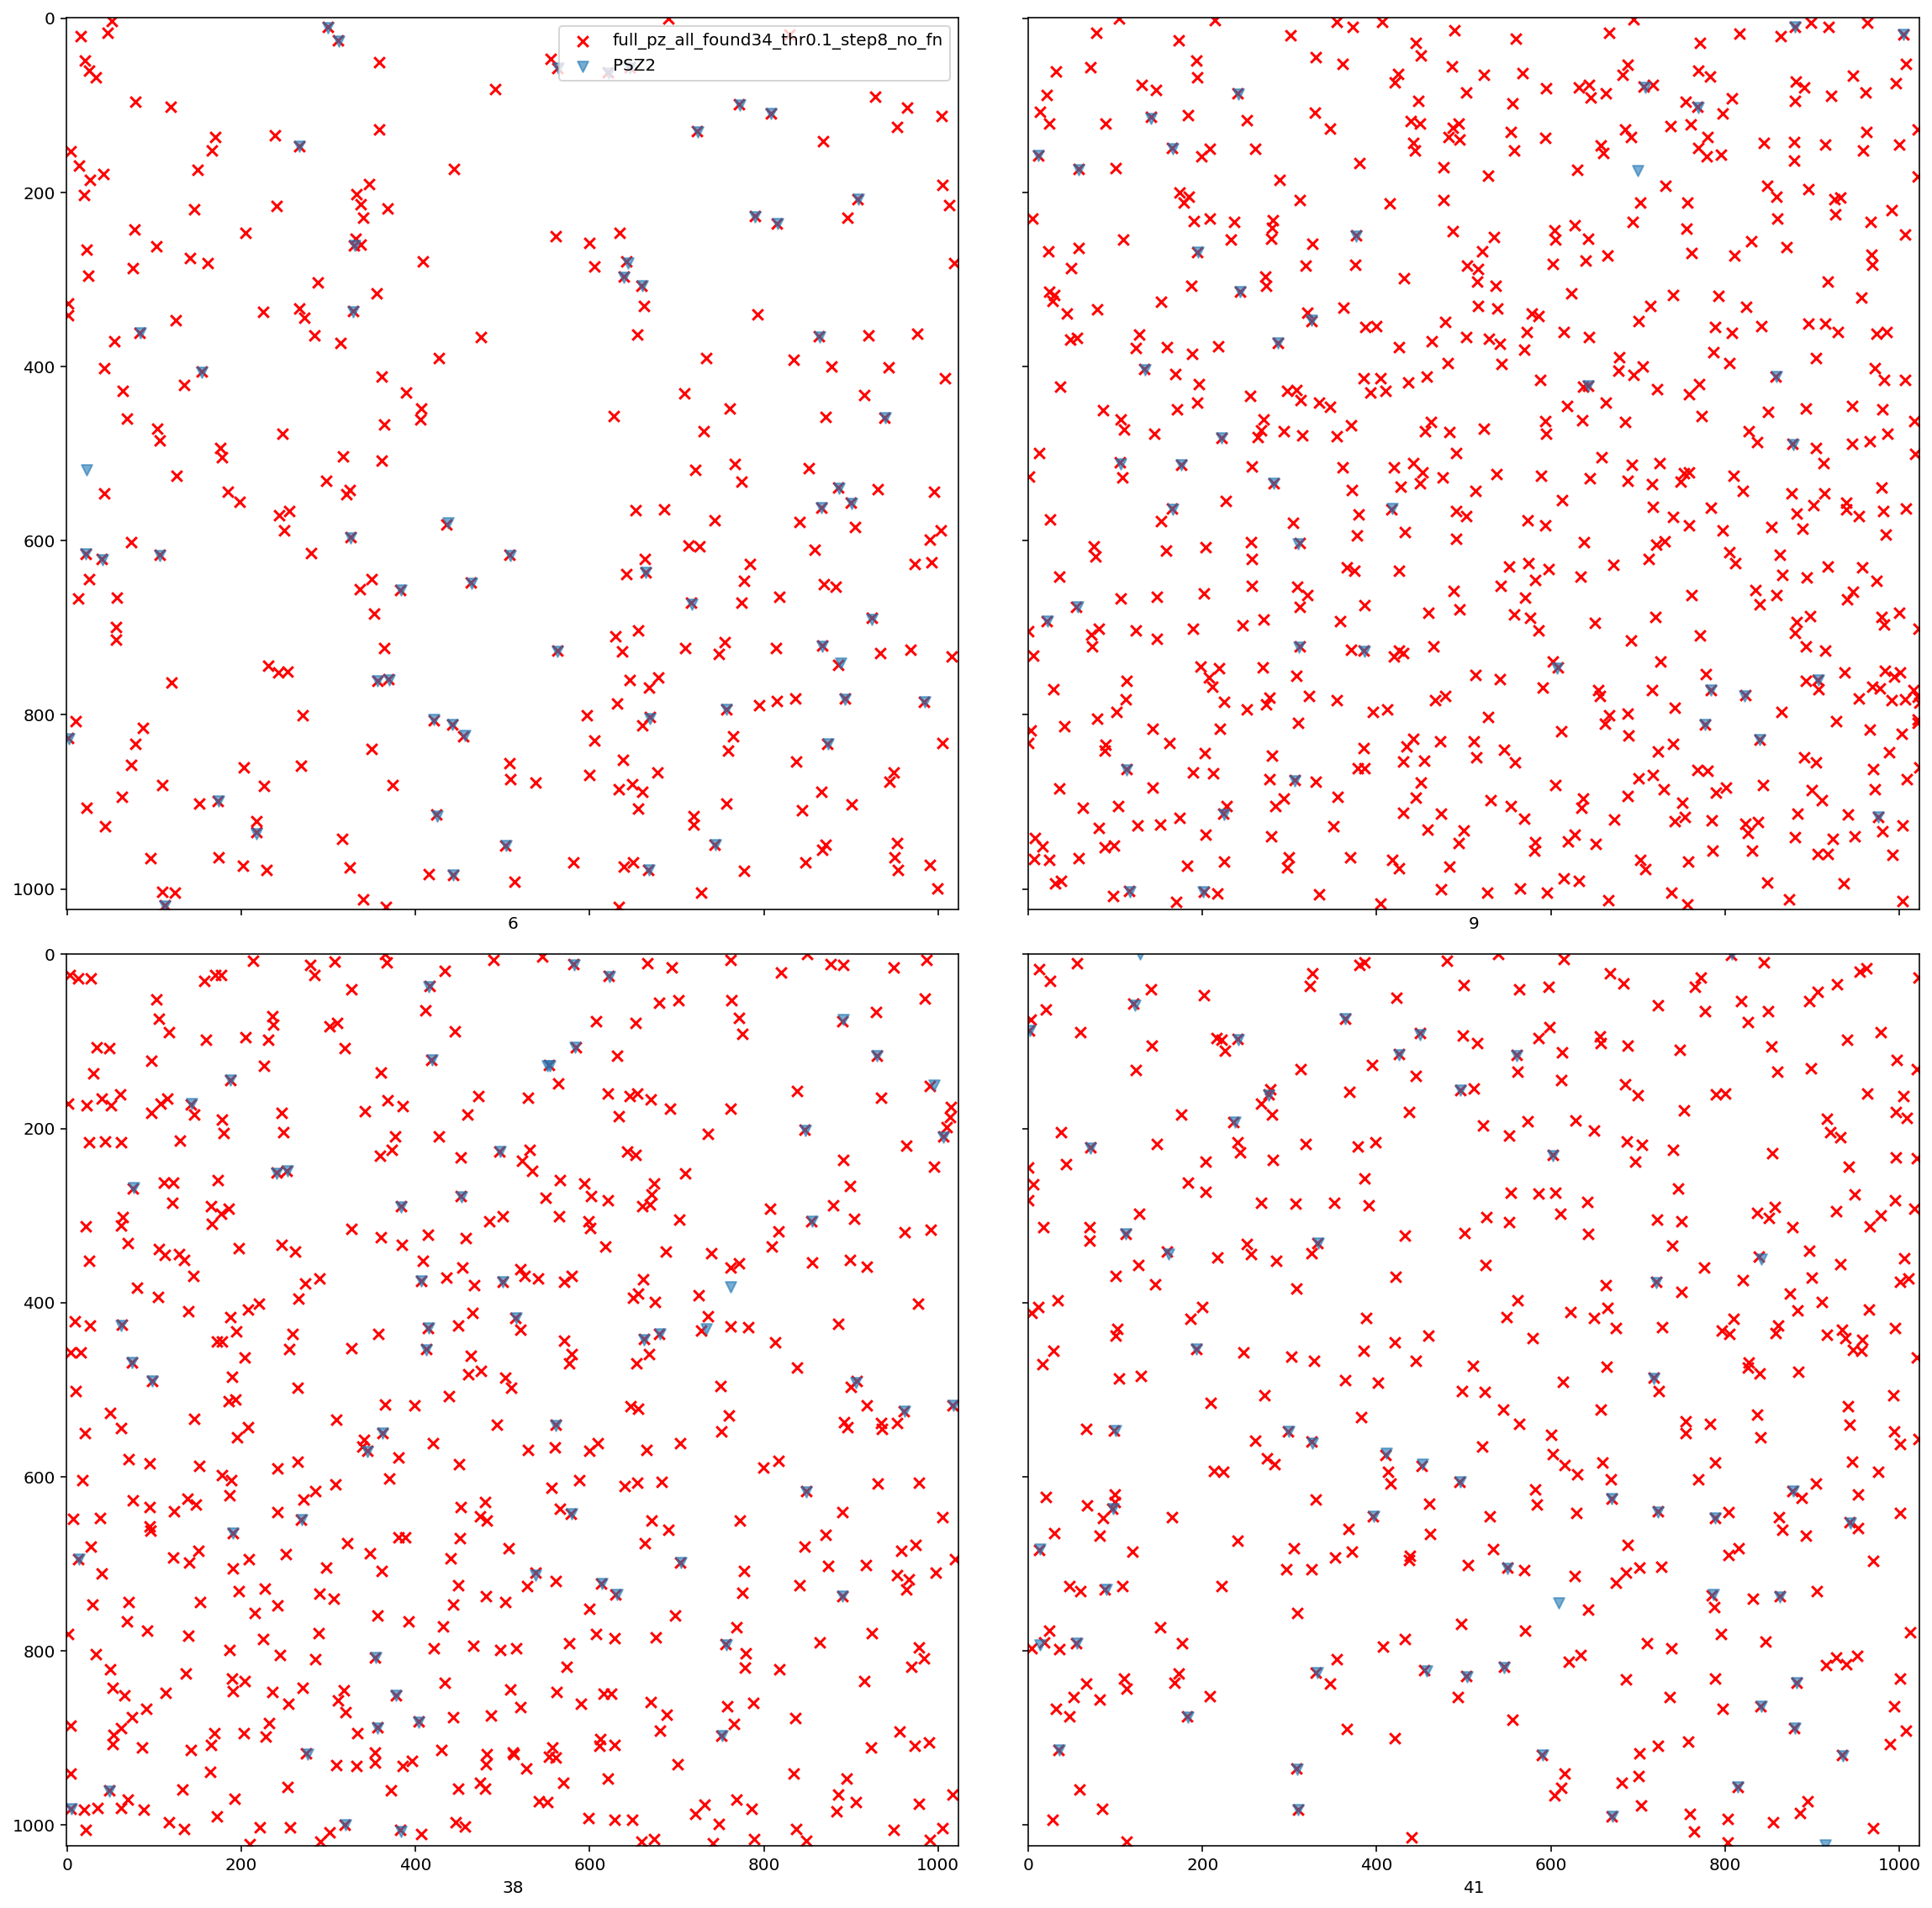
\includegraphics[width=\linewidth]{map_psz2}
\caption{Карта распределения объектов из детектированного каталога и скоплений из ground truth 
    каталогов (PSZ2), пиксели из разбиения $n_{side}=2$ с номерами
    $[6, 38]$ (левая колонка - восток) и $[9, 41]$ (правая колонка - запад)}
\label{Fig:Map_PSZ2}
\end{figure}

\begin{figure}[h]
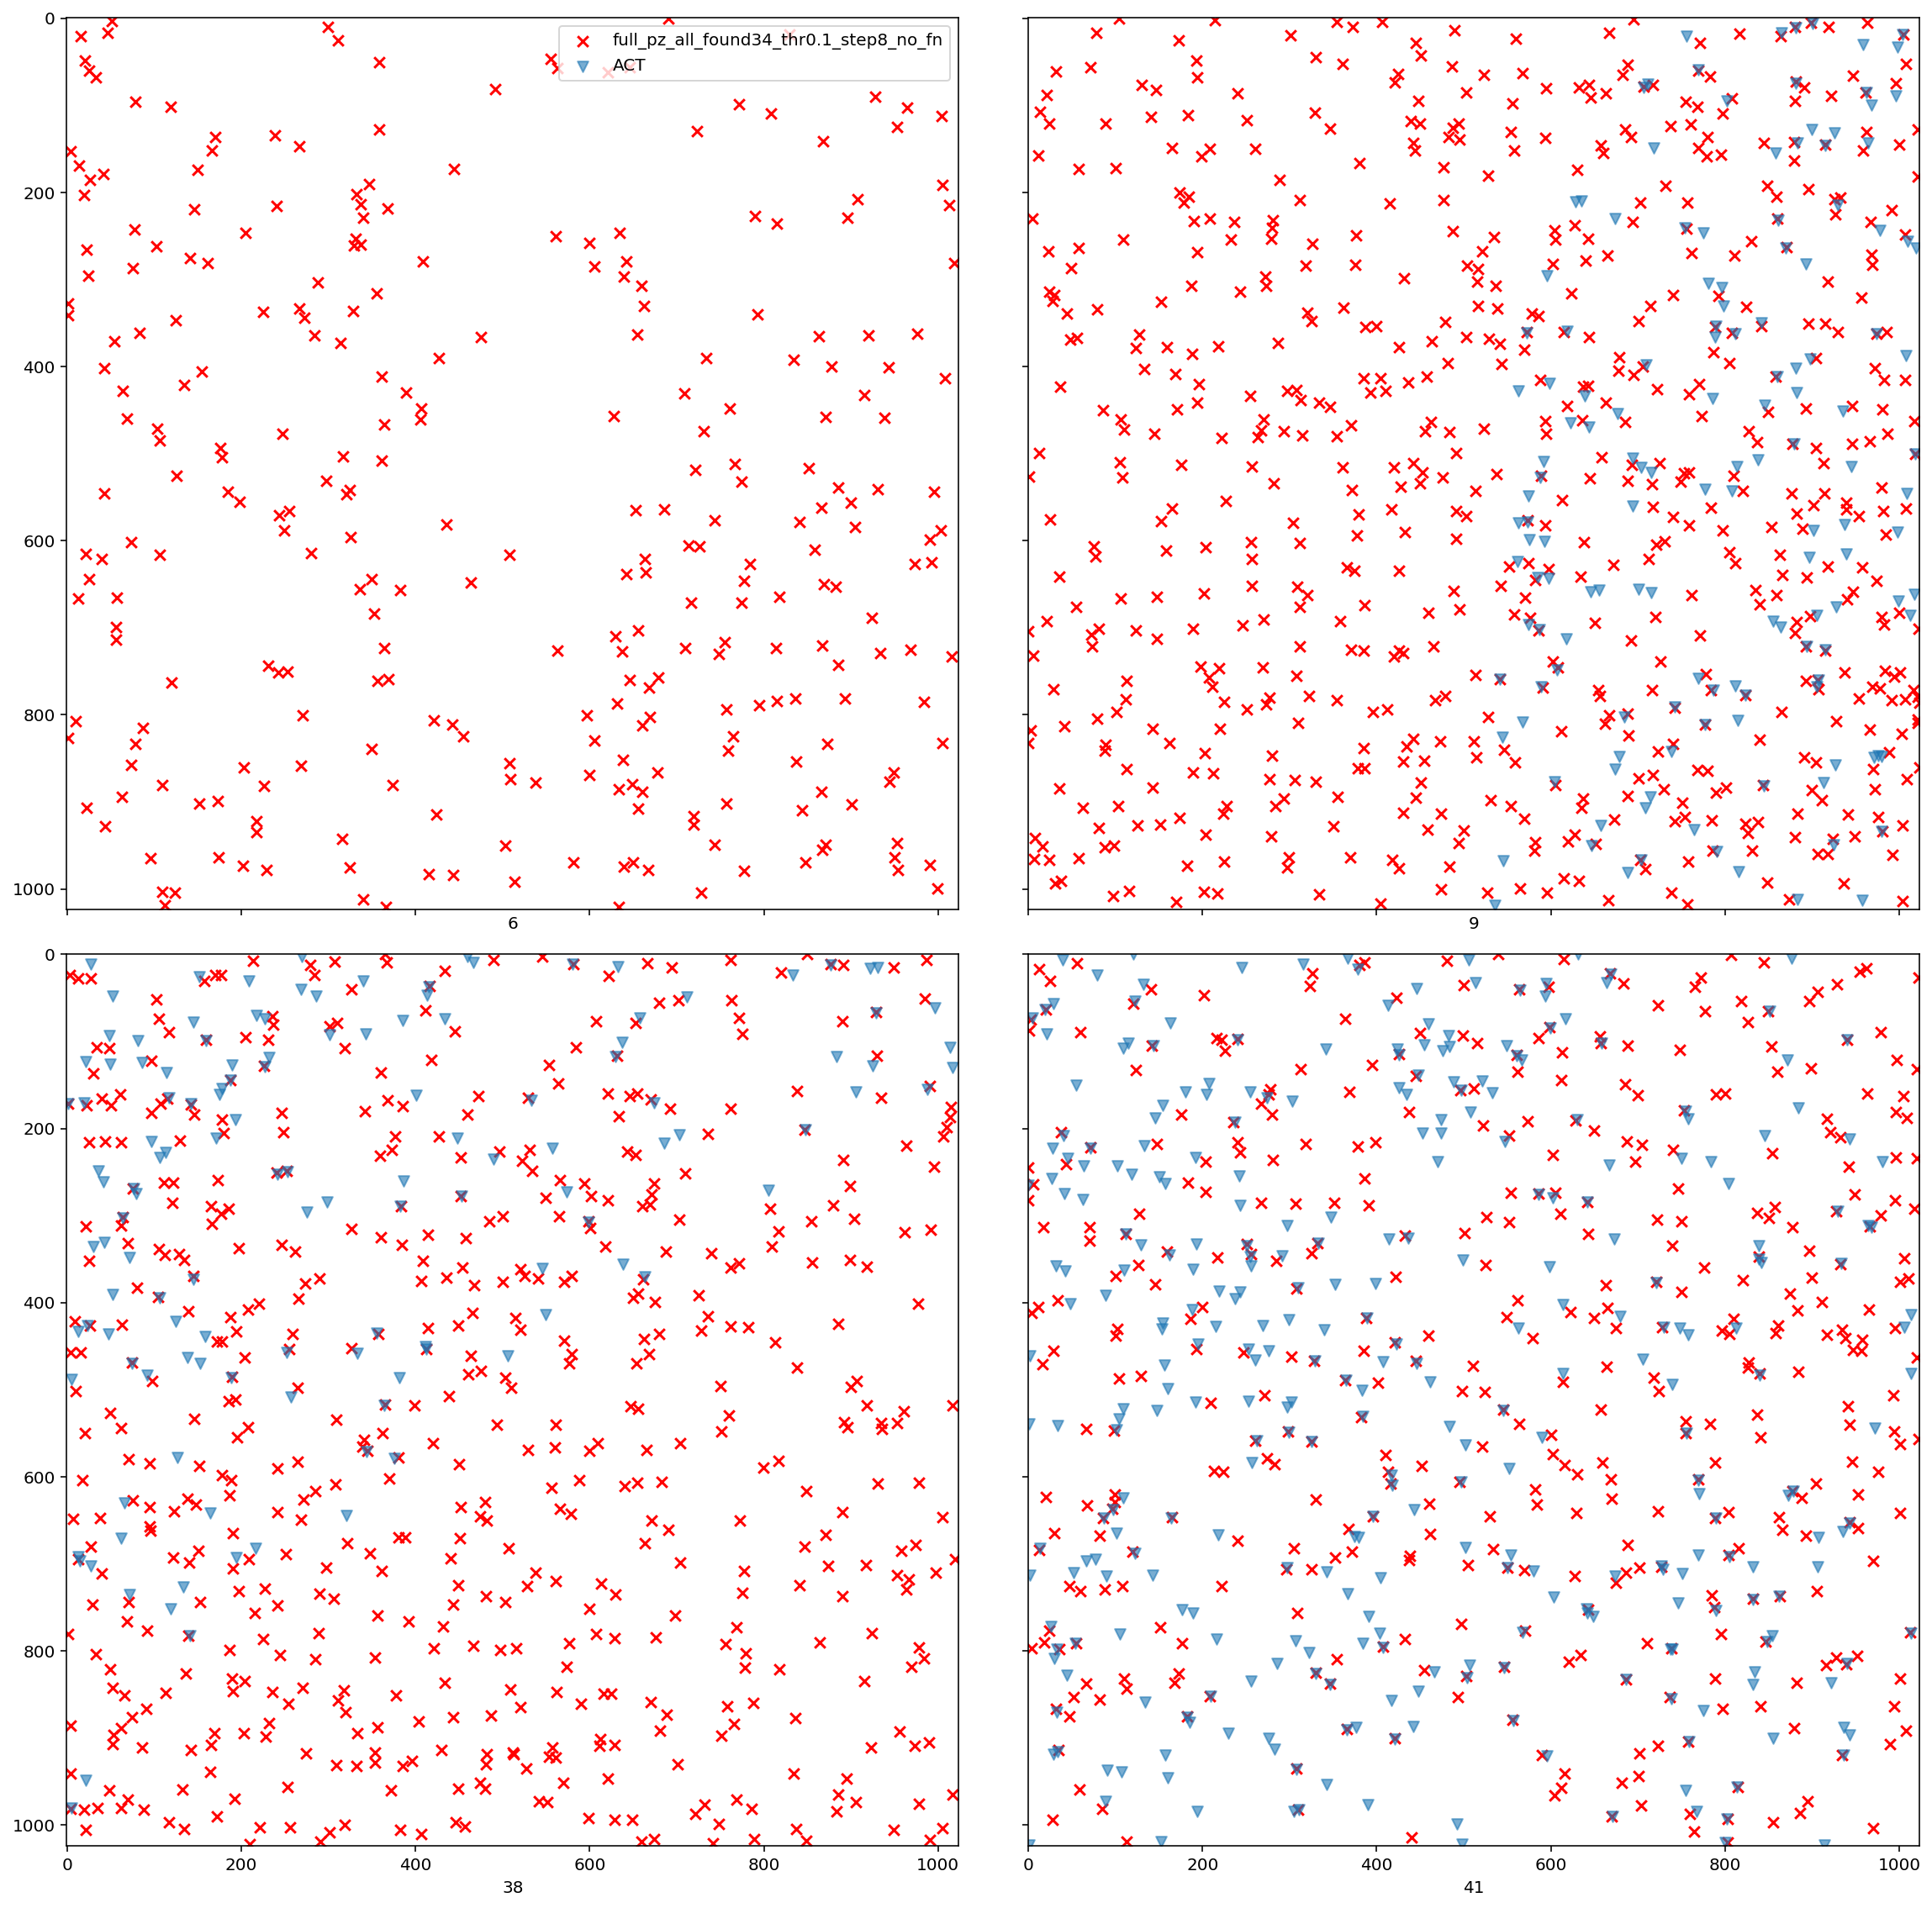
\includegraphics[width=\linewidth]{map_act}
\caption{Карта распределения объектов из детектированного каталога и скоплений из ground truth 
    каталогов (ACT), пиксели из разбиения $n_{side}=2$ с номерами
    $[6, 38]$ (левая колонка - восток) и $[9, 41]$ (правая колонка - запад)}
\label{Fig:Map_ACT}
\end{figure}
Отчет согласован с научным руководителем.\\
Общее количество строк кода за эту неделю: 158\\
\href{https://github.com/rt2122/data-segmentation-2}{Репозиторий}\\ 
\end{document}
